\documentclass[12pt]{article}

\usepackage{hyperref}
\usepackage{graphicx}
\usepackage{enumitem}
\usepackage{xepersian}

\settextfont{Vazirmatn}
\linespread{1.3}

\author{متین اعظمی}
\author{محمد حسینی}
\author{عسل خائف}
\author{ارشیا شفیعی}
\author{شیدا عابدپور}
\author{امیرعلی لطفی}
\author{زهرا معصومی}
\title{سامانه کارا}

\begin{document}

	\begin{figure}
		\centering
		
\includegraphics[width=0.3\textwidth]{files/logo}
	\end{figure}
	\begin{center}
		دانشگاه اصفهان\\
		دانشکده مهندسی کامپیوتر
		\vspace{2\baselineskip}

		{\Huge \textbf{سامانه کارا}}\\

		\vspace{1\baselineskip}
		کاریابی هدفمند در سازمان‌ها، شرکت‌ها و صنایع\\
		\vspace{2\baselineskip}
		\textbf{پدیدآورندگان به ترتیب الفبا:}\\
		متین اعظمی\\
		محمد حسینی\\
		عسل خائف\\
		ارشیا شفیعی\\
		شیدا عابدپور\\
		امیرعلی لطفی\\
		زهرا معصومی\\

		\vspace{1\baselineskip}
		{\textbf{استاد راهنما:}}
		 دکتر محمدرضا شعرباف\\
		\vspace{2\baselineskip}
		ترم پاییز 1401

	\end{center}
	\newpage
	\tableofcontents
	\newpage

	\section{سند تبیین نیازمندی‌ها}

	\subsection{مقدمه}
	در این بخش به تبیین نیازمندی‌های سیستم می‌پردازیم که در قالب استاندارد 1998-830
	\textbf{Std IEEE}
	 بیان شده است.
	با توجه به افزایش روز افزون مسئله کاریابی، نیاز به بستری برای تسهیل و تسریع این فرایند حس می‌شود. بدیهی است که مدیریت این فرایند و اطمینان یافتن از درست طی شدن آن نیاز به برنامه‌ریزی دقیقی دارد.
	در این پروژه سامانه‌ای طراحی شده است که علاوه بر کمک به کارجویان جهت کاریابی آسان‌تر و جلوگیری از مراجعه حضوری به دفاتر کاریابی و استفاده از روش‌های سنتی، کمک به کارفرمایان جهت استخدام دقیق و بهتر کارجویان خود را در نظر داشته باشد.


	\subsubsection{هدف}
	سند تبیین نیازمندی‌های نرم‌افزار و یا به اختصار
	\textbf{SRS}
	، سندی است که در آن به شرح کامل جزئیات نیازمندی‌های سیستم، طریقه ارتباط آنها با سیستم و یا با یکدیگر، عوامل تاثیرگذار بر سیستم، واسط‌های گوناگونی که در بخش‌های مختلف سیستم به کار رفته است و کارکرد محصول از جنبه‌های مختلف می‌پردازد.
	به طور خلاصه، این سند دیدی جامع از محصول را به نمایش می‌گذارد و به سه گروه از افراد کمک می‌کند و نیازمندی‌های آن‌ها به دست آمده است:

	\begin{enumerate}
		\item
		\textbf{کارجویان:}
		این سند نشان‌ دهنده آن است که کارجو از سیستم چه انتظاراتی دارد و چه نیازمندی‌هایی باید برای این انتظارات در نظر گرفته شود. این کار باعث شده کارجو درک بهتری از نیازهای خود پیدا کرده و نیازهایش را مدیریت کند.
		\item
		\textbf{کارفرمایان:}
		این سند نشان دهنده آن است که کارفرما از سیستم چه انتظاراتی دارد و جهت تسهیل و تسریع روند استخدام چه نیازمندی‌هایی باید برای او در نظر گرفته شود. این کار باعث شده کارفرما درک بهتری از نیاز‌های خود پیدا کرده و آن‌ها را مدیریت کند.
		\item
		\textbf{مدیر سیستم:}
		این دسته از افراد نیز همانند کارجویان و کارفرمایان، باید دید کلی و جامعی از نیازمندی‌های سیستم داشته باشند. لذا این سند یک توافق اولیه میان کارجو و کارفرما و مدیر سیستم برای آنچه سیستم باید انجام دهد، به وجود می‌آورد و حلال مشکلات بسیاری خواهد بود.
	\end{enumerate}
	همچنین در آغاز پروژه به کمک این سند می‌توان پیش‌بینی اولیه‌ای از وضعیت زمان‌بندی و هزینه‌های پروژه انجام داد.

	\subsubsection{قلمرو}
	 این پروژه یک سیستم نرم‌افزاری است که به هدف سرعت بخشیدن و بهبود فرایند کاریابی برنامه‌ریزی شده است.
	این سامانه، تحت عنوان "\textbf{کارا}" جهت ثبت آگهی، معرفی شرکت‌های مطرح، انجام آزمون‌های شخصیتی، ساخت رزومه مناسب، تخمین حقوق، ایجاد بستر ارتباط مجازی برای ایجاد پلی بین کارجو و کارفرما و هر قابلیتی که از نظر گروه به بهبود روند کاریابی به کارجو و کارفرما کمک می‌کند، طراحی شده است.
	انتظار می‌رود که این سامانه بتواند با دریافت مشخصات معتبر و احراز هویت، در فضایی امن، امکان استفاده کاربران از امکانات تارنما را به آن‌ها بدهد و در حیطه استخدام و کاریابی به کارفرمایان و کارجویان کمک شایانی کند.
	در این سامانه تا آنجایی که امکان داشته طراحی به صورتی انجام شده که عوام جامعه هم بتوانند با آن کار کنند، همچنین سعی شده تا محدودیت‌های افراد با شرایط خاص نیز در نظر گرفته شود. با این حال سامانه امکان بهبود و توسعه جهت بهتر شدن را دارد ولی به دلیل محدودیت زمانی موجود به بخش‌های اشاره شده در فوق بسنده کرده‌ایم.

	\subsubsection{تعاریف، سرنام‌ها و کوته‌نوشت‌ها}
		\begin{itemize}
		\item
		\textbf{SRS}
		کوته‌شده عبارت
		\lr{Specification Requirement Software}
	 	  است.
		\item
		\textbf{IEEE}
		کوته‌شده عبارت
		\lr{Institute of Electrical and Electronics Engineers}
		  است.
		\item
		\textbf{STD}
		 کوته‌شده واژه
		 \r{Standard}
		  است.
		\item
		\textbf{HTTPS}
		 کوته‌شده عبارت
		\lr{Hyper Text Transfer Protocol Secure}
		است که یک \textbf{پروتکل} ارتباطی برای انتقال امن اطلاعات در شبکه‌های کامپیوتری است که به صورت خاص در اینترنت استفاده می‌شود.
		\item
		\textbf{SSL}
		کوتاه‌شده عبارت
		\lr{Secure Socket Layer}
		 است که پروتکلی است برای ردّ و بدل کردن سندهای خصوصی از طریق اینترنت.
		\item
		\textbf{HTML}
		یک زبان نشانه‌گذاری است که کوته‌شده واژه
		\lr{HyperText Markup Language}
		است.
		\item
		\textbf{CSS}
		کوتاه شده عبارت
		\lr{Cascading Style Sheets}
		 است.
		\item
		\textbf{جاوا اسکریپت:}
		\lr{JavaScript}
		 (به اختصار \lr{JS})
		 یک زبان برنامه نویسی است که برای توسعه نرم‌افزارهای مرتبط با وب استفاده می‌شود.
		\item
		\textbf{مرورگر وب:}
		 نوعی نرم‌افزار کاربردی است که برای دریافت، نمایش، مرور و ارسال اطلاعات، جستجوی تارنماها در وب جهانی یا یک تارنمای محلی مورد استفاده قرار می‌گیرد.
		\item
		\textbf{پروتکل:}
		 به معنی مجموعه‌ای از قوانین و رویه‌ها برای برقراری ارتباط است.
		\item
		\textbf{سیستم عامل:}
		 نرم‌افزار سیستمی‌ای است که مدیریت منابع رایانه را به عهده گرفته و بستری را فراهم می‌سازد که نرم‌افزار کاربردی اجرا شده و از خدمات آن استفاده کنند.
		\item
		\textbf{سرور ابری:}
		یک نوع سرور می‌باشد که در رایانش ابری ایجاد شده و بر روی بستر اینترنت برای بسیاری از کاربران ارائه می‌شود.
		\item
		\textbf{Web Server:}
		نرم‌افزاری کامپیوتری است که اصلی‌ترین وظیفه آن ارائه اطلاعات و سرویس‌های درخواست شده در قالب صفحات وب به کاربران است.
		\item
		\textbf{PDF}
		 کوته‌شده عبارت
		\lr{Portable Document Format}
		  است.
		\item
		\textbf{JPG/JPEG}
		کوته‌شده عبارت
		\lr{Joint Photographic Expert Group}
		  است.
		\item
		\textbf{SSD}
		 کوته‌شده‌ عبارت
		\lr{Solid-State Drive}
		  است.
		\item
		\textbf{Captcha}
		کوته‌شده عبارت
		\lr{Completely Automated Public Turing test to tell Computers and Humans Apart}
	 	 می‌باشد.
		\item
		\textbf{رمزنگاری:}
		ابزاری است که برای انتقال و نگه‌داری امن اطلاعات استفاده می‌شود. در واقع هدف رمزنگاری این است که داده را به گونه‌ای نگه‌داری یا ارسال کند که فقط کسانی که مجاز هستند، به اصل داده‌ها دسترسی داشته باشند.
		\item
		\textbf{یادگیری ماشین:}‌
		 معادل آن
		\lr{Machine Learning}
		 است که مطالعه‌ی الگوریتم‌ها و مدل‌های آماری مورد استفاده‌ی سیستم‌های کامپیوتری است که به‌جای استفاده از دستورالعمل‌های واضح، از الگوها و استنباط برای انجام وظایف استفاده می‌کنند.
		\item
		\textbf{رابط کاربری گرافیکی:}
		یک محیط گرافیکی که نرم‌افزارهای رایانه، برای راهنمایی و کاربری بهتر انسان بکار می‌گیرند.
		\item
		\textbf{طراحی واکنش‌گرا:‌}
		رابط کاربری گرافیکی‌ای که با تغییر اندازه صفحات، نوع چیدمان عناصر در صفحه را تغییر دهد.
		\item
		\textbf{کاربر‌پسند:}
		ویژگی نرم‌‏افزار یا سخت‏‌افزاری که کار کردن با آن و یادگیری استفاده از آن، برای کاربران تازه‏‌کار یا بی‌‏تجربه، ساده و آسان باشد.
		\item
		\textbf{مودم:}
		یک از ابزار رایانه‌ای است که برای اتصال دو رایانه به یکدیگر و شبکه‌های مختلف از راه خطوط گوناگون مخابراتی استفاده می‌شود.
		\item
		\textbf{کارت شبکه:‌}
		سخت‌افزار رایانه به صورت کارتی در شیارهای توسعه مادربورد رایانه قرار می‌گیرد و رایانه را به شبکه متصل می‌کند.
		\item
		\textbf{پایگاه‌داده:}
		مجموعه‌ای سازمان یافته از داده‌های ذخیره شده و الکترونیکی است.
		\item
		\textbf{سیستم مدیریت پایگاه‌داده:}
		معادل عبارت
		 \lr{Database Management System}
		 یا به اختصار DBMS است که نرم‌افزاری است که از مجموعه‌ای از ابزارها و بخش‌های مرتبط با هم به منظور فراهم آوردن امکان مدیریت کامل اطلاعات ذخیره شده در پایگاه‌داده تشکیل شده است.
		\item
		\textbf{دستیار صوتی:}
		 یک عامل نرم‌افزاری است که با صوت به کاربر کمک می‌کند از سیستم استفاده کند.
		\item
		\textbf{کیو-آر کد}
		 کوته‌شده عبارت
		 \lr{Quick-Response Code}
		  و معادل فارسی آن "رمزینه پاسخ سریع" می‌باشد که یک رمزینه ماتریسی است که دربردارنده چیدمانی از نقطه‌های مربع‌شکل سیاه‌رنگ (با نام ماژول) بر روی زمینه سفید است. داده نهفته می‌تواند نوشته، نشانی وب، پیامک، شماره تلفن، اطلاعات کارت ویزیت یا داده دیگری باشد.
		\item
		\textbf{تارنوشت:}
		  نوعی وبگاه است که حاوی اطلاعاتی مانند: گزارش روزانه، اخبار، یادداشت‌های شخصی یا مقالات علمی مورد نظر طراح آن است. در این سیستم تارنوشت به منظور انتشار نویسه‌های مدیر سیستم ایجاد شده است.
		\item
		\textbf{نویسه‌ تارنوشت:}
		یک نوشته در تارنوشت است. معادل انگلیسی آن
		\lr{Blog Post}
		 می‌باشد.
		\item
		\textbf{شخص حقیقی:}
		 هر انسانی که زنده است و در جامعه زندگی می‌کند یک شخص حقیقی نامیده می‌شود که این شخص دارای شخصیت و حقوق مخصوص به خود می‌باشد.
		\item
		\textbf{شخص حقوقی:}
		 هر سازمان، نهاد، وزارتخانه یا مؤسسه‌ای است که فعالیت تجاری یا غیر‌تجاری خاصی را انجام می‌دهد.
		\item
		\textbf{کارجو:}
		 یک شخص حقیقی است که به دنبال استخدام می‌باشد.
		\item
		\textbf{کارفرما:}
		 یک شخصیت حقیقی یا شخصیت حقوقی است که به دنبال استخدام کارجو در موقعیت شغلی‌های  می‌باشد.
		\item
		\textbf{شرکت:}
		 هر سازمان، نهاد، یا مو‌ٔسسه‌ای که توسط یک کارفرما در سیستم ثبت شده باشد.
		\item
		\textbf{پشتیبان تارنما:}
		شخصی حقیقی که وظیفه کمک و راهنمایی کاربران را به منظور استفاده از سیستم دارد.
		\item
		\textbf{پست الکترونیک معتبر:}
		 هر رشته که ساختار درست یک پست الکترونیک را داشته باشد.
		\item
		\textbf{وضعیت روند رزومه:}
		هر رزومه ارسال شده در سیستم، در یکی از وضعیت‌های زیر قرار خواهد داشت:
		\begin{itemize}
			\item
			\textbf{ارسال شده:}
			وضعیت اولیه هر رزومه است که به معنای ارسال موفقیت آمیز رزومه از سمت کارجو به سمت کارفرما می‌باشد.
			\item
			\textbf{‌مشاهده شده توسط کارفرما:}
			رزومه توسط کارفرما دیده شده است؛ ولی هنوز تأیید نشده است.
			\item
			\textbf{در دست بررسی:}
			رزومه در اولویت بررسی سازمان قرار گرفته است و کارشناسان سازمان در حال بررسی بیشتر بر روی رزومه هستند.
			\item
			\textbf{تایید اولیه:}
			 مرحله بررسی با موفقیت پشت سر گذاشته شده است و کارفرما رزومه را تایید اولیه کرده است.
			\item
			\textbf{دعوت به مصاحبه:}
			کارفرما پس از تایید اولیه، کارجو را به مصاحبه دعوت کرده است.
			\item
			\textbf{رد شده:}
			رزومه توسط کارفرما به هر دلیل رد شده است.
			\item
			\textbf{منجر به استخدام:}
			کارفرما پس از انجام مصاحبه، کارجو را استخدام کرده است.
			\item
			\textbf{لغو توسط کارجو:}
			کارجو درخواست استخدام خود را لغو کرده است و رزومه دیگر برای کارفرما نمایش داده نمی‌شود.
			\item
			\textbf{منقضی شده:}
			اگر کارفرما پس از گذشت ۴۵ روز از ارسال رزومه،‌ وضعیت نهایی آن را مشخص نکند، رزومه به این وضعیت تغییر می‌کند.
			\item
			\textbf{آگهی بسته شده:}
			اگر آگهی مربوطه بسته شده باشد، رزومه در هر وضعیتی که باشد به این وضعیت تغییر می‌کند.
		\end{itemize}
		\item
		\textbf{آزمونک‌های صحت‌سنجی:}
		 آزمونک‌هایی که توسط سیستم به صورت آنلاین برای هر کارجو برگزار می‌شود و صحت تسلط کارجو بر یک مهارت را ارزیابی می‌کند.
		\item
		\textbf{توصیه‌نامه:}
		 یک فایل الکترونیکی به فرمت PDF که در آن یک کارجو برای کار در یک موقعیت شغلی توصیه شده است.
		\item
		\textbf{اشتراک ویژه:}
		کاربران سیستم با پرداخت هزینه‌‌‌، اشتراک ویژه سیستم را تهیه می‌کنند که با این اشتراک مجموعه‌ای از قابلیت‌های سیستم برای آن‌ها فعال می‌شود.
		\item
		\textbf{اسناد و اطلاعات محرمانه:}
		این اسناد شامل هر مدرک ارسالی توسط کارجویان و کارفرمایان و اطلاعات وارد شده آن‌ها در سیستم می‌باشد.
		\item
		\textbf{سیستم پیشنهاد دهنده موقعیت‌های شغلی:}
		یک عامل نرم‌افزاری است که با استفاده از داده‌های جمع‌آوری شده از سوی یک کارجو نظیر سوابق جستجو، رزومه، و آگهی‌های نشان شده، موقعیت‌های شغلی جدید مناسب آن کارجو را به دست می‌آورد و به کارجو پیشنهاد می‌دهد.
		\item
		\textbf{تالار گفتگو:}
		یک محیط مجازی است که کاربران سیستم می‌توانند به صورت آنلاین در آن با یکدیگر به گفتگو بپردازند.
		\item
		\textbf{گفتگو سریع با پشتیبان:}
		هر کاربر در سیستم از طریق این ویژگی می‌تواند به صورت آنلاین با پشتیبان سامانه در ارتباط باشد.
		\item
		\textbf{ماشین حساب حقوق:}
		یک عامل نرم‌افزاری است که با پردازش بر روی داده‌های وارد شده از سوی دیگر کاربران، که شامل عنوان شغلی؛ سطح ارشدیت؛ سابقه کاری؛ حقوق دریافتی می‌باشد، می‌تواند با دریافت عنوان شغلی، سطح ارشدیت و سابقه کاری یک کاربر، یک حقوق تخمین زده شده پیشنهادی اعلام کند.
		\item
		\textbf{وزارت صمت:}
		 سرواژه "وزارت صنعت، معدن و تجارت".
		\item
		\textbf{نماد شرکت:}
		 هر تصویر که نشانگر هویت یک سازمان می‌باشد.
		\item
		\textbf{پیش‌نویس آگهی:}
		یک نسخه منتشر نشده از آگهی شغلی که فقط برای کارفرمای مربوطه قابل مشاهده می‌باشد.
		\item
		\textbf{تور مجازی:‌}
		نمایش فضاهای مختلف به صورت ۳۶۰ درجه و فراگیر به بینندگان بوده و با شبیه‌سازی حضور بازدیدکننده در فضای مربوطه جزئیات متعددی از آن فضا را به تصویر می‌کشد.
		\item
		\textbf{یادگیری عمیق:}
		\lr{Deep Learning}
		  بخشی از روش‌های یادگیری ماشین است که بر روش‌هایی تمرکز دارد که مبتنی بر شبکه‌های عصبی مصنوعی هستند. یادگیری عمیق به رایانه‌ها می‌آموزد آنچه را که به طور طبیعی برای انسان انجام می‌شود، انجام دهند.
		\item
		\textbf{سیستم های توصیه کننده:}
		\lr{Recommender Systems}
		  با تحلیل رفتار کاربر خود، اقدام به پیشنهاد مناسب‌ترین اقلام (داده، اطلاعات، کالا و…) می‌نماید.
		\item
		\textbf{خوشه‌بندی:}
		\lr{Clustering}
		 گروه‌بندی مجموعه‌ای از اشیاء انجام می‌شود، اینکار به این صورت است که اشیاء در یک گروه (به نام خوشه) در مقایسه با دیگر دسته‌ها (خوشه‌ها) مشابه‌تر هستند.
		\item
		\textbf{تشخیص گفتار:}
		\lr{Speech Recognition}
		  به معنای استفاده از رایانه و هوش مصنوعی برای تشخیص کلمات و عبارت موجود در صوت انسان و تبدیل آنها به متن به عنوان خروجی است.
		\item
		\textbf{پردازش زبان‌های طبیعی:}
		\lr{Natural Language Processing}
		 عبارت است از استفاده از رایانه برای پردازش زبان گفتاری و زبان نوشتاری. بدین معنی که رایانه‌ها را قادر سازیم که گفتار یا نوشتار تولید شده در قالب و ساختار یک زبان طبیعی را تحلیل و درک نموده یا آن را تولید نمایند.
		\item
		\textbf{چت جی‌پی‌تی:}
		\lr{Chat GPT}
		 به معنای
		\lr{Generative Pre-trained Transformer}
		 از مدل‌های زبانی هستند که عموماً بر روی مجموعه بزرگی از داده‌های متنی آموزش داده شده‌اند تا متنی شبیه انسان تولید کنند. آنها با استفاده از چندین بلوک از معماری ترانسفورماتور ساخته شده اند.
	\end{itemize}
	\subsubsection{مراجع}
	\begin{itemize}
		\item
		کونگ، دیوید سی: مهندسی نرم‌افزار شئ‌گرا (یک متدولوژی چابک یکنواخت) جلد اوّل. ترجمه: دکتر بهمن زمانی و دکتر افسانه فاطمی، ۱۳۹۴.
		\item
		Charles Edeki, International Journal of Computer Science and Mobile Applications, Vol.1 Issue. 3, September- 2013, pg. 13-17.
		\item
		{lr}{IEEE Std 830-1998 IEEE Recommended Practice for Software Requirements Specifications, In IEEE Xplore Digital Library.\\
		http://ieeexplore.ieee.org/Xplore/guesthome.jsp }
		\item
		Software engineering: a practitioner's approach, Pressman, Roger S. Palgrave macmillan, 2005.

	\end{itemize}

	\subsubsection{طرح کلی}
	سلام1

	\subsection{شرح کلی}
	\subsubsection{چشم‌انداز محصول}
	\subsubsection{کارکرد محصول}
	\subsubsection{مشخصات کاربر}
	\subsubsection{قیود و محدودیت‌ها}
	\subsubsection{مفروضات و وابستگی‌ها}

	\subsection{نیازمندی‌های خاص}
	\subsubsection{نیازمندی‌های کارکردی}
	\subsubsection{نیازمندی‌های کارایی}
	\subsubsection{نیازمندی‌های واسط خارجی}
	\subsubsection{قیود طراحی}
	\subsubsection{صفات سیستم نرم‌افزاری}

		\begin{enumerate}
			\renewcommand{\labelenumi}{R\arabic{enumi}}
			\item First item
			\item Second item
			\begin{enumerate}
			\renewcommand{\labelenumii}{R\arabic{enumi}.\arabic{enumii}}
			\item First subitem
			\item Second subitem
			\end{enumerate}
		\item Third item
	\end{enumerate}

	\section{قوانین کسب و کار}
	sgghl

	\section{برنامه تکرار و برنامه مرحله}
	sghl 3

	\begin{figure}
		\centering
		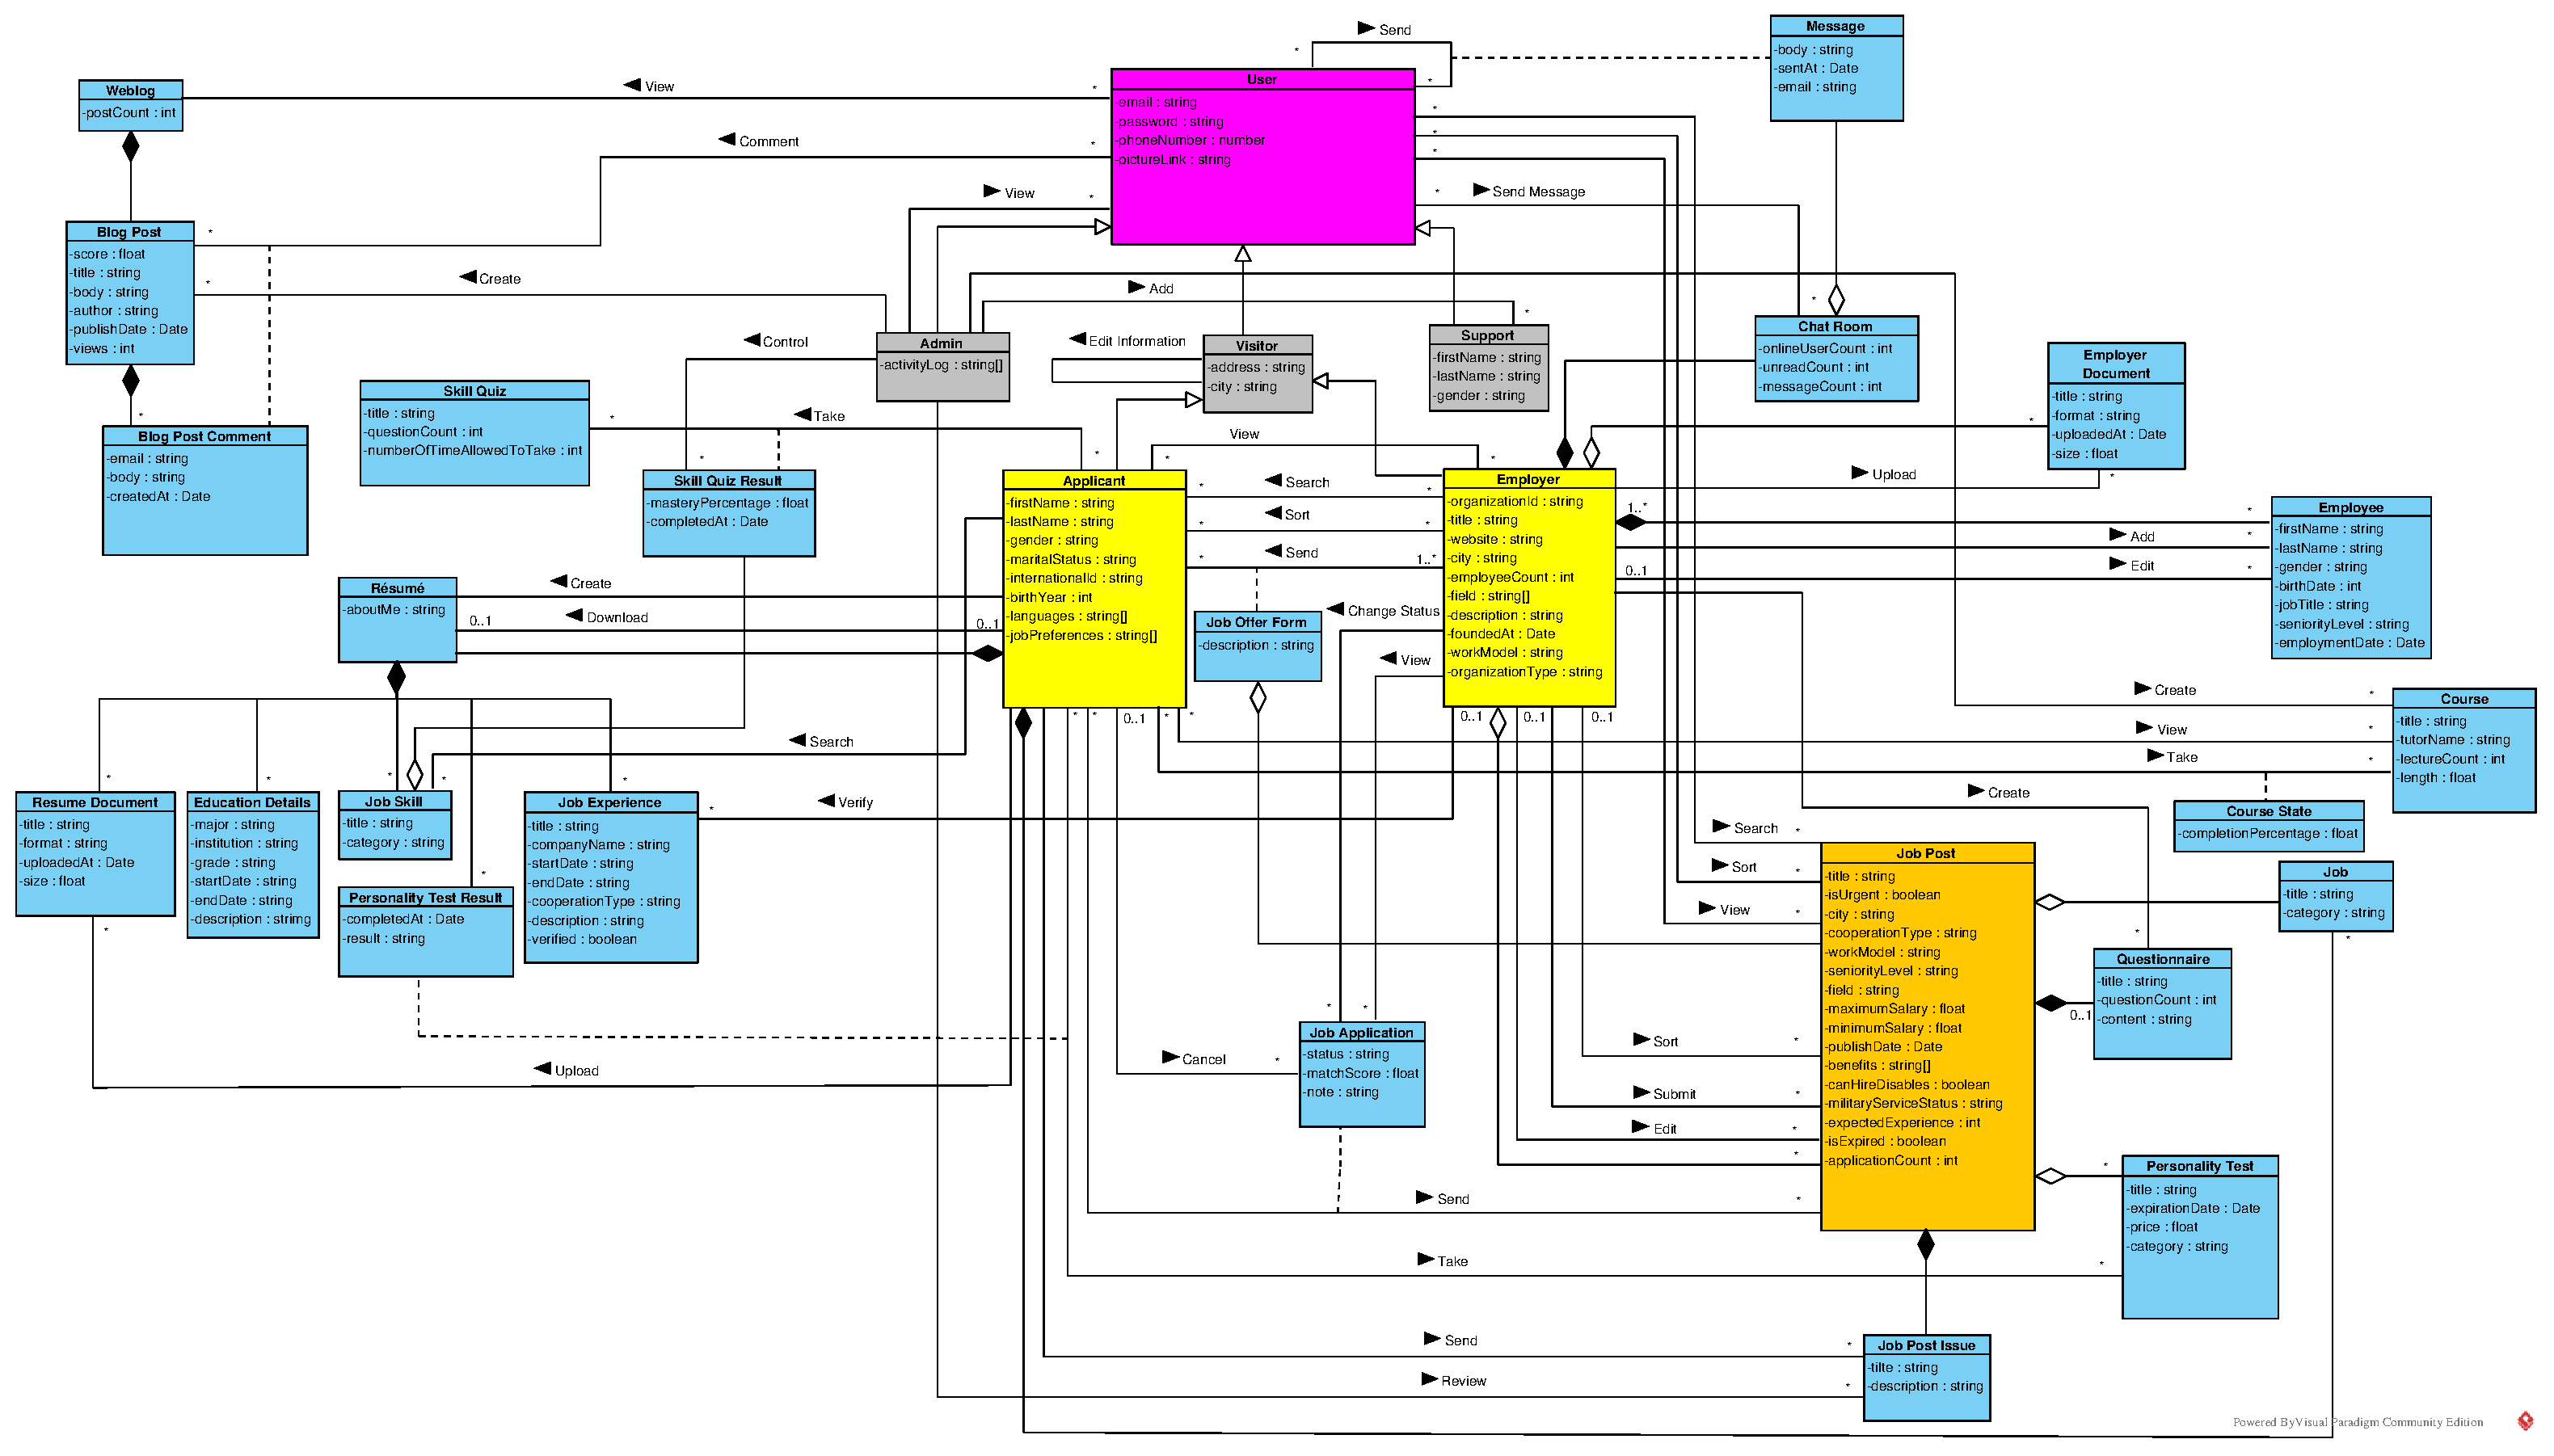
\includegraphics[width=1.5\linewidth]{files/Project_OOAD_Phase2_DiagramClass_V5_EnglishVersion}
		\caption{}
		\label{fig:projectooadphase2diagramclassv5englishversion}
	\end{figure}



	\section{مدل‌سازی دامنه}

	\section{طراحی معماری}

	\section{استخراج موردکابردها و مدل‌سازی تعامل کنشگر-سیستم}

	\begin{itemize}
		\item First item
		\item Second item
		\item Third item
	\end{itemize}

	\begin{enumerate}
		\renewcommand{\labelenumi}{.R\arabic{enumi}}
		\item First item
		\item Second item
		\begin{enumerate}
			\renewcommand{\labelenumii}{.R\arabic{enumi}.\arabic{enumii}}
			\item First subitem
			\item Second subitem
		\end{enumerate}
		\item Third item
	\end{enumerate}


\end{document}